\documentclass{article}\usepackage[]{graphicx}\usepackage[]{xcolor}
% maxwidth is the original width if it is less than linewidth
% otherwise use linewidth (to make sure the graphics do not exceed the margin)
\makeatletter
\def\maxwidth{ %
  \ifdim\Gin@nat@width>\linewidth
    \linewidth
  \else
    \Gin@nat@width
  \fi
}
\makeatother

\definecolor{fgcolor}{rgb}{0.345, 0.345, 0.345}
\newcommand{\hlnum}[1]{\textcolor[rgb]{0.686,0.059,0.569}{#1}}%
\newcommand{\hlstr}[1]{\textcolor[rgb]{0.192,0.494,0.8}{#1}}%
\newcommand{\hlcom}[1]{\textcolor[rgb]{0.678,0.584,0.686}{\textit{#1}}}%
\newcommand{\hlopt}[1]{\textcolor[rgb]{0,0,0}{#1}}%
\newcommand{\hlstd}[1]{\textcolor[rgb]{0.345,0.345,0.345}{#1}}%
\newcommand{\hlkwa}[1]{\textcolor[rgb]{0.161,0.373,0.58}{\textbf{#1}}}%
\newcommand{\hlkwb}[1]{\textcolor[rgb]{0.69,0.353,0.396}{#1}}%
\newcommand{\hlkwc}[1]{\textcolor[rgb]{0.333,0.667,0.333}{#1}}%
\newcommand{\hlkwd}[1]{\textcolor[rgb]{0.737,0.353,0.396}{\textbf{#1}}}%
\let\hlipl\hlkwb

\usepackage{framed}
\makeatletter
\newenvironment{kframe}{%
 \def\at@end@of@kframe{}%
 \ifinner\ifhmode%
  \def\at@end@of@kframe{\end{minipage}}%
  \begin{minipage}{\columnwidth}%
 \fi\fi%
 \def\FrameCommand##1{\hskip\@totalleftmargin \hskip-\fboxsep
 \colorbox{shadecolor}{##1}\hskip-\fboxsep
     % There is no \\@totalrightmargin, so:
     \hskip-\linewidth \hskip-\@totalleftmargin \hskip\columnwidth}%
 \MakeFramed {\advance\hsize-\width
   \@totalleftmargin\z@ \linewidth\hsize
   \@setminipage}}%
 {\par\unskip\endMakeFramed%
 \at@end@of@kframe}
\makeatother

\definecolor{shadecolor}{rgb}{.97, .97, .97}
\definecolor{messagecolor}{rgb}{0, 0, 0}
\definecolor{warningcolor}{rgb}{1, 0, 1}
\definecolor{errorcolor}{rgb}{1, 0, 0}
\newenvironment{knitrout}{}{} % an empty environment to be redefined in TeX

\usepackage{alltt}
\IfFileExists{upquote.sty}{\usepackage{upquote}}{}
\begin{document}



\section{Chapter 2. Theoretical Foundations of Data Visualisation}
In the realm of data science, the power of data visualisation is undeniable. The ability to transform raw data into compelling visual representations not only enables us to see patterns and trends but also serves as a bridge for effective communication of empirical findings. To harness this potential to its fullest, it is crucial to lay down a solid theoretical foundation that underpins the art and science of data visualisation.\\

This chapter, "Theoretical Foundations of Data Visualisation," delves deep into the core principles and concepts that serve as the bedrock of this dynamic field. We seek to understand not only the "how" but also the "why" behind the creation of visualisations that captivate and inform.

\section{Chapter 2.1. Introduction to Data Visualisation Theory}
In the pursuit of creating effective data visualisations, it is crucial to understand that behind every compelling chart, graph, or map lies a solid theoretical framework. Theoretical underpinnings provide the foundation upon which data visualisation is built, shaping not only how we represent data but also how we perceive, understand, and interpret it. 


\subsection{2.1.1 Guiding Principles for Data Representation}
Within this theoretical framework, we encounter a set of guiding principles that dictate how data should be represented visually. These principles encompass fundamental concepts such as:
\begin{itemize}
    \item \textbf{Accuracy}: Data visualisations should accurately reflect the underlying data, minimising distortion or misinterpretation.
    \item \textbf{Simplicity}: The "less is more" principle applies to data visualisation. Simplified visuals often convey information more effectively than cluttered ones.
    \item \textbf{Clarity}: Visualisations should be clear and understandable to the intended audience, avoiding unnecessary complexity.
    \item \textbf{Relevance}: Information presented should be relevant to the message or question being addressed.
    \item \textbf{Consistency}: Visual elements, such as colour coding and labelling, should be used consistently throughout a visualisation.
\end{itemize}

\subsection{2.1.2 Theoretical Framework and Visual Perception}
One of the fundamental aspects of data visualisation theory is an understanding of how the human brain perceives visual information. This knowledge is instrumental in designing visualisations that resonate with viewers. It includes considerations like:
\begin{itemize}
    \item \textbf{Gestalt Principles}: The Gestalt principles of visual perception, including proximity, similarity, and continuity, influence how we group and interpret visual elements in a visualisation.
    \item \textbf{Colour Theory}: The effective use of colour, including colour contrasts and harmonies, can enhance the clarity and impact of a visualisation.
    \item \textbf{Cognitive Load}: Minimising the mental effort required to process information is vital.
\end{itemize}

\section{Chapter 2.2 Visual Perception and Cognition}
Understanding the intricacies of how humans interpret visual information is pivotal to the art and science of data visualisation. Thus, we explore human visual perception, along with the application of cognitive psychology principles in data visualisation and highlight the crucial role of pre-attentive attributes in shaping our perception of data. 

\subsection{2.2.1 Human Visual Perception: Decoding Visual Information
}
Human visual perception is a remarkable cognitive process that allows us to decode and make sense of the world around us. When applied to data visualisation, it illuminates how viewers interact with and derive meaning from visual representations of data. Key aspects of human visual perception in the context of data visualisation include:
\begin{itemize}
    \item \textbf{Pattern Recognition}: The human brain excels at recognizing patterns, making it adept at identifying trends, outliers, and relationships in data visualisations.
    \item \textbf{Perceptual Grouping}: We tend to group visually similar elements together, a principle known as perceptual grouping. This informs how we interpret clusters of data points and shapes in a visualisation.
    \item \textbf{Hierarchy of Perception}: Certain visual attributes are processed more quickly and efficiently than others. For example, colour is often processed faster than text, influencing the viewer's attention hierarchy.
\end{itemize}

By harnessing the principles of human visual perception, applying insights from cognitive psychology, and leveraging pre-attentive attributes, data visualisation designers can create visualisations that are not only aesthetically pleasing but also cognitively efficient.	

\section{Chapter 2.3 Gestalt Principles}
Gestalt psychology principles have long been recognised as fundamental to the field of visual perception and design. In this section, we provide an overview of Gestalt principles, delve into their relevance in the context of data visualisation, and explore how these principles can be applied to create more effective and intuitive visualisations.

\subsection{2.3.1 Overview of Gestalt Psychology Principles}
Gestalt psychology is a school of thought that emphasises how humans perceive and organise visual information. It posits that the mind seeks to create meaningful patterns and wholes from individual visual elements. The Gestalt principles provide a framework for understanding how viewers naturally group and interpret visual stimuli.

\subsection{2.3.2 Key Gestalt Principles and Their Relevance}
Several key Gestalt principles play a pivotal role in shaping our perception of visual information. These principles include: 
\begin{itemize}
    \item \textbf{Proximity}: Elements that are close to each other are perceived as related or belonging to the same group. In data visualisation, proximity can be used to group data points or related information.
    \item \textbf{Similarity}: Elements that share similar visual attributes, such as colour, shape, or size, are perceived as belonging together. Similarity can be harnessed to encode categorical data or highlight relationships.
    \item \textbf{Continuity}: The human mind tends to perceive continuous patterns or lines as a single entity. In data visualisation, continuity can aid in representing trends or connections between data points.
    \item \textbf{Closure}: Viewers tend to mentally complete incomplete shapes or patterns. Closure can be employed to suggest relationships or connections even when not explicitly shown in the visualisation.
    \item \textbf{Symmetry}: Symmetrical elements are often perceived as more balanced and harmonious. Symmetry can be used for aesthetically pleasing and easily understandable visualisations.
\end{itemize}

\subsection{2.3.3 Application of Gestalt Principles in Designing Visualisations}
The application of Gestalt principles in designing data visualisations can lead to more intuitive and effective communication of information. Designers can strategically leverage these principles to:
\begin{itemize}
    \item Group-related data points to enhance clarity and reduce visual clutter.
    \item Use colour or shape to signify meaningful categories or groupings.
    \item Create smooth, continuous lines or paths to guide the viewer's gaze through the visualisation.
    \item Suggest connections or patterns even in complex datasets.
\end{itemize}

\section{Chapter 2.4 Data abstraction and Representation}
The transformation of raw data into meaningful representations is a pivotal step in data visualisation. This process, known as data abstraction, involves distilling complex datasets into visual forms that convey insights. In this section, we explore data abstraction, the hierarchies and levels of abstraction in data visualisation, and the critical trade-offs between abstraction and the potential loss of information.

\subsection{2.4.1 Data Abstraction: Transforming Raw Data}
Data abstraction is the art of simplifying and structuring raw data into formats that are comprehensible and insightful. It is the bridge that transforms numbers, text, and variables into visual elements that convey patterns, trends, and relationships. Effective data abstraction is at the heart of creating informative data visualisations.

\subsection{2.4.2 Hierarchies and Levels of Abstraction}
In data visualisation, abstraction operates on multiple levels of granularity. Hierarchies of abstraction allow us to represent data at varying levels of detail: 
\begin{enumerate}
    \item \textbf{Low-Level Abstraction}: At the lowest level, raw data is preserved in its most detailed form. This might include individual data points, measurements, or unprocessed text.
    \item \textbf{Mid-Level Abstraction}: As we move up the hierarchy, data is grouped or aggregated to provide a broader overview. For example, hourly data points may be aggregated into daily or weekly averages.
    \item \textbf{High-Level Abstraction}: At the highest level, data is represented in a condensed and abstracted form, often as summary statistics or key insights. This level provides a big-picture view.
\end{enumerate}

\subsection{2.4.3 Trade-offs Between Abstraction and Information Loss}
While abstraction is essential for simplifying complex data, it comes with trade-offs. Increasing levels of abstraction can lead to information loss, where fine-grained details or outliers are overlooked. It is crucial for data visualisation designers to strike a balance:
\begin{itemize}
    \item \textbf{Clarity vs. Detail}: Increasing abstraction can enhance the clarity of a visualisation but may sacrifice detailed information that is important for certain analytical tasks.
    \item \textbf{Generalisation vs. Specificity}: Abstraction can provide a more generalised view of data, making it accessible to a wider audience. However, it may miss specific nuances that experts may require.
    \item \textbf{Context vs. Precision}: High-level abstraction can provide valuable context, but it may lack the precision needed for precise decision-making.
\end{itemize}
In data visualisation, the art of data abstraction lies in finding the right level of detail that effectively conveys the intended message while minimising the risk of information loss. This balancing act is a critical consideration in the design of informative and meaningful data visualisations.

\section{Chapter 2.5 Data Types and Visualisation Techniques}
In the world of data visualisation, understanding the nature of your data is key. Data comes in various types, and selecting the appropriate visualisation technique is contingent upon recognising these distinctions. In this section, we categorise data types, and demonstrate how to match each data type with suitable visualisation techniques.

\subsection{2.5.1 Categorisation of Data Types}
Data types can be broadly categorised into four main types: 
\begin{itemize}
    \item \textbf{Nominal data}: nominal data represents categories or labels without any inherent order. Examples include colours, gender categories, and city names. 
    \item \textbf{Ordinal data}: ordinal data implies a meaningful order or ranking among categories but lacks equal intervals between them. Examples include survey responses (eg. “very satisfied”, “satisfied”, “neutral”, “dissatisfied”, “very dissatisfied”)
    \item \textbf{Interval data}: interval data possesses ordered categories with equal intervals between them, but it lacks a true zero point. Temperature is measured in Celsius or Fahrenheit as an example. 
    \item \textbf{Ratio data}: ratio data includes ordered categories with equal intervals and a meaningful zero point. Examples are age, income, and weight. 
\end{itemize}

\subsection{2.5.2 Matching Data Types with Appropriate Visualisation Techniques}
Selecting the right visualisation technique for your data type is pivotal to effective communication. Here are some examples of visualisation techniques matches with corresponding data types: 
\begin{itemize}
    \item \textbf{Nominal data}: Techniques such as bar charts and stacked bar charts are effective in displaying categorical information and relative proportions. 
    \item \textbf{Ordinal data}: Ordinal data can be visualised using ordered bar charts, dot plots, or stacked bar charts, which maintain the ranking and order of the categories.
    \item \textbf{Interval data}: Interval data benefits from visualisation methods like line charts, histograms, and box plots, which highlight trends and distributions without assuming a true zero point. 
    \item \textbf{Ratio data}: Ratio data can be effectively presented using scatter plots, histograms, and line charts, allowing for precise comparisons and measurements due to the presence of a meaningful zero point. 
\end{itemize}

\section{Chapter 2.6 Colour Theory in Data Visualisation}
Here, we explore the significance of colour in data visualisation, the principles of colour perception and encoding, and the importance of avoiding misleading visualisations through thoughtful colour choices.

\subsection{2.6.1 The Importance of Colour in Conveying Information}
Colour is a potent tool for enhancing the understanding and impact of data visualisations. It enables the differentiation of data points, highlights trends, and provides context. Colour can be used to:
\begin{itemize}
    \item \textbf{Encode Categorical Data}: Distinguish between different groups or classes using distinct colours.
    \item \textbf{Represent Quantitative Data}: Use colour intensity or gradients to represent values or magnitudes.
    \item \textbf{Add Context}: Apply colour to background elements, labels, or annotations to provide context and meaning to the visualisation.
\end{itemize}

\subsection{2.6.2 Colour Perception and Colour Encoding in Visualisations}
Understanding how colour is perceived by viewers is essential in data visualisation. Key principles include:
\begin{itemize}
    \item \textbf{Colour Discrimination}: Consider that not all viewers may perceive colour in the same way. Ensure your colour choices are accessible to individuals with colour vision deficiencies (colour blindness).
    \item \textbf{Colour Encoding}: Select colour schemes that align with the message you want to convey. For example, warm colours like red and orange often signify caution or heat, while cool colours like blue and green convey calmness or coldness.
    \item \textbf{Colour Combinations}: Pay attention to how colours interact when placed adjacent to each other. Some combinations may create visual vibrations or make text difficult to read.
\end{itemize}

\subsection{2.6.3 Avoiding Misleading Visualisations Due to Colour Choices}
Misleading visualisations can result from inappropriate or deceptive use of colour. To avoid this:
\begin{itemize}
    \item \textbf{Consistency}: Maintain consistency in colour usage throughout your visualisation. Use the same colour scheme for similar data categories or elements.
    \item \textbf{Avoid Distortion}: Ensure that colour choices do not exaggerate or distort the data. Overly intense or contrasting colours can lead to misinterpretation.
    \item \textbf{Legend Clarity}:  Provide a clear and concise legend to explain the meaning of colours, especially when dealing with complex or unfamiliar colour schemes. 
    \item \textbf{Test with Users}: Conduct user testing to ensure that your colour choices effectively convey the intended message and do not confuse or mislead the audience.
\end{itemize}

\\
In summary, colour theory is a critical component of data visualisation. Thoughtful colour choices can enhance the clarity and impact of visualisations, making data more accessible and understandable. However, it is equally important to use colour judiciously to avoid misleading visualisations and ensure that the message remains accurate and informative.

\section{Chapter 2.7 Theoretical Properties of Visualisations}
Effective data visualisation is not solely about creating aesthetically pleasing graphics; it's also about adhering to key theoretical properties that optimise the expressiveness, precision, accuracy, and scalability of visual representations. In this section, we delve into these properties, including expressiveness and effectiveness, the data-ink ratio, and the principles of minimal ink, as well as precision, accuracy, and scalability.

\subsection{2.7.1 Expressiveness and Effectiveness}
\begin{itemize}
    \item \textbf{Expressiveness}: Visualisations should be expressive, meaning they should effectively communicate the intended message or insights within the data. Expressive visualisations capture the richness and complexity of the underlying data, revealing patterns, trends, and relationships.
    \item \textbf{Effectiveness}: An effective visualisation is one that successfully conveys information to its audience. It allows viewers to understand the data, draw meaningful conclusions, and make informed decisions based on the presented information.
\end{itemize}

\subsection{2.7.2 Data-Ink Ratio and the Principle of Minimal Ink} REVISE
This \textbf{Data-Ink Ratio principle}, introduced by Edward Tufte REFERENCEEEEEEEEEE, emphasises maximising the ink (or pixels in digital formats) used to represent the actual data while minimising non-essential ink. A higher data-ink ratio results in a cleaner, more efficient visualisation that reduces clutter and enhances comprehension.\\
The \textbf{Principle of Minimal Ink} REFERENCEEEEEEEEE builds on the data-ink ratio. This principle advocates for the removal of any visual elements that do not contribute to the viewer's understanding of the data. Eliminating unnecessary ink (e.g., excessive gridlines or decorations) simplifies the visualisation without sacrificing its effectiveness.

\subsection{2.7.3 Precision, Accuracy, and Scalability}
\begin{itemize}
    \item \textbf{Precision}: Precision in data visualisation refers to the level of detail and granularity in the representation of data. Visualisations should strike a balance between showing enough detail to support accurate interpretation while avoiding overwhelming viewers with excessive complexity.
    \item \textbf{Accuracy}: Accuracy pertains to how faithfully the visualisation represents the true values in the data. Misleading or distorted visualisations can lead to incorrect conclusions. Therefore, maintaining accuracy is essential.
    \item \textbf{Scalability}: Scalability addresses how well a visualisation adapts to different data sizes or resolutions. Effective visualisations should be scalable, and capable of representing both small and large datasets without sacrificing clarity or performance.
\end{itemize}

\section{Chapter 2.8 Cognitive Load and Visual Complexity}
In data visualisation, achieving a balance between complexity and cognitive load is crucial. This section explores the concept of cognitive load in visualisations, strategies to reduce cognitive load while maintaining complexity, and techniques to combat information overload through simplification.

\subsection{2.8.1 Exploring the Concept of Cognitive Load in Visualisations}
In data visualisations, cognitive load plays a significant role in how viewers engage with and understand the presented data. It is essential to strike a balance that ensures the visualisation conveys information effectively without overwhelming or overtaxing the viewer's cognitive capacity.

\subsection{2.8.2 Strategies to Reduce Cognitive Load While Maintaining Complexity}
\begin{itemize}
    \item \textbf{Visual Hierarchy}: Establish a clear visual hierarchy that guides viewers' attention to the most important elements of the visualisation. Use techniques such as size, colour, and contrast to emphasise key information.
    \item \textbf{Simplify Labels and Text}: Reduce cognitive load by using concise labels and text. Avoid jargon and unnecessary complexity in annotations, ensuring that labels are informative and straightforward.
    \item \textbf{Interactive Features}: Implement interactive elements, such as tooltips and drill-down functionality, to provide additional information when viewers need it, reducing the need for dense, static visualisations.
    \item \textbf{Progressive Disclosure}: Present complex information gradually, allowing viewers to digest it in stages. Start with an overview and provide opportunities for users to explore details as needed.
    \item \textbf{Data Aggregation}: Consider aggregating data when it makes sense. Summarising data can reduce the cognitive load associated with interpreting fine-grained details.
\end{itemize}

\subsection{2.8.3 Information Overload and Simplification Techniques}
Information overload occurs when a visualisation overwhelms viewers with excessive data or visual elements, hindering comprehension. To combat information overload, the following simplification techniques can be applied:
\begin{itemize}
    \item \textbf{Filtering}: Allow viewers to filter data based on specific criteria, enabling them to focus on the most relevant information.
    \item \textbf{Data Reduction}:  Aggregate or summarise data to present overarching trends or patterns instead of inundating viewers with raw data points.
    \item \textbf{Studyboarding}: Use storytelling techniques to guide viewers through the data in a structured manner, helping them understand the context and relevance of the information presented.
    \item \textbf{Prioritisation}: Identify the most critical information and prioritise its display, relegating less essential data to secondary views or interactions.
\end{itemize}






\section{Chapter 3. Modern Methods of Data Visualisation}

\section{Chapter 3.1 Introduction to Modern Data Visualization Methods}
xxx

\section{Chapter 3.2 Scatter Plots and Bubble Charts}
Scatter plots and bubble charts are fundamental data visualization techniques that provide valuable insights into the relationships and patterns within datasets. These visualizations are particularly effective for representing data points, making comparisons, and revealing trends. Below, we delve into the characteristics, use cases, and advantages of scatter plots and bubble charts.

\subsection{Scatter Plots}
A scatter plot is a simple yet powerful visualization that displays individual data points as dots on a two-dimensional plane. Each point represents a unique data entry, with one variable on the horizontal (x-axis) and another on the vertical (y-axis). Scatter plots are versatile and can accommodate various data types, including nominal, ordinal, interval, and ratio.

\subsubsection{Advantages}
\begin{itemize}
    \item Easy identification of patterns and trends. 
    \item Effective for outlier detection. 
    \item Suitable for both bi-variate and multi-variate analysis.
    \item Offers a visual representation of the distribution of data points.
\end{itemize}

\subsection{Scatter Plots in Practice}
In this example, we'll create a scatter plot that visualizes the relationship between two variables while adding colors, labels, and a trend line for added interest. We'll use the built-in "mtcars" R dataset, which contains information about various car models.

\begin{knitrout}
\definecolor{shadecolor}{rgb}{0.969, 0.969, 0.969}\color{fgcolor}\begin{kframe}


{\ttfamily\noindent\itshape\color{messagecolor}{\#\# `geom\_smooth()` using formula = 'y \textasciitilde{} x'}}\end{kframe}
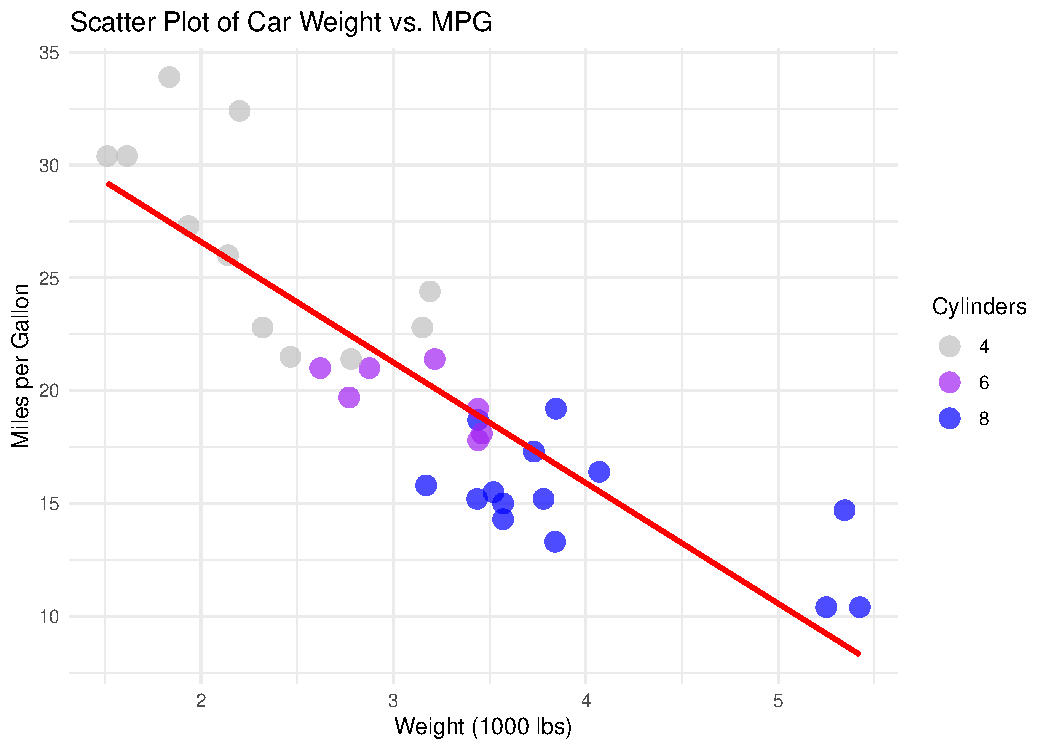
\includegraphics[width=\maxwidth]{figure/scatter-plot-chunk-1} 
\end{knitrout}

\subsubsection{Analysis} TO BE REVISED
The scatter plot displays the relationship between car weight (in thousands of pounds, "wt") and fuel efficiency (miles per gallon, "mpg") for different car models from the "mtcars" dataset. Here are the key characteristics of the plot:
\begin{itemize}
    \item Color-Coded Cylinders: The points are color-coded based on the number of cylinders in the engine (4, 6, and 8 cylinders). This allows for a quick visual differentiation of car types, enhancing the understanding of the data.
    \item Point Size and Transparency: Points are larger in size and have some degree of transparency (alpha) for visual appeal. Larger, more prominent points are easier to see, while transparency helps in the visualization of overlapping points.
    \item Linear Regression Line: A blue linear regression trend line is included. It provides a visual representation of the overall relationship between car weight and fuel efficiency, indicating a negative correlation—cars tend to have lower fuel efficiency as their weight increases.\\
\end{itemize}
    
\subsection{Why a Scatter Plot is Appropriate}
A scatter plot is an appropriate choice for this dataset and analysis for the following reasons:\\

1. Relationship Visualization: A scatter plot is well-suited for showing the relationship between two continuous variables, such as car weight and fuel efficiency. It allows us to visually assess the pattern and direction of the relationship.

2. Regression Line: The inclusion of a regression line provides a clear summary of the overall trend, highlighting the negative correlation between car weight and fuel efficiency.
EXPLAIN REGRESSION


\subsection{Bubble Charts}
A bubble chart is an extension of the scatter plot, where each data point is represented as a bubble or circle. In addition to the x and y axes, bubble charts introduce a third variable that is encoded by the size of the bubbles. This third variable allows for the simultaneous visualization of three data attributes.

\subsection{Use Cases}
Bubble charts are particularly useful when you need to visualize the relationship between three variables. For example, in finance, a bubble chart can display the market capitalization, price-to-earnings ratio, and stock returns for different companies simultaneously. In public health, it can represent the population, vaccination coverage, and disease incidence for various regions.

\subsubsection{Advantages}
\begin{itemize}
    \item Visualising three data attributes in a single chart.
    \item Easily conveying the magnitude of the third variable through bubble size.
    \item Effective for exploring complex relationships and identifying patterns. 
\end{itemize}

\subsection{Bubble Charts in Practice}
\begin{knitrout}
\definecolor{shadecolor}{rgb}{0.969, 0.969, 0.969}\color{fgcolor}
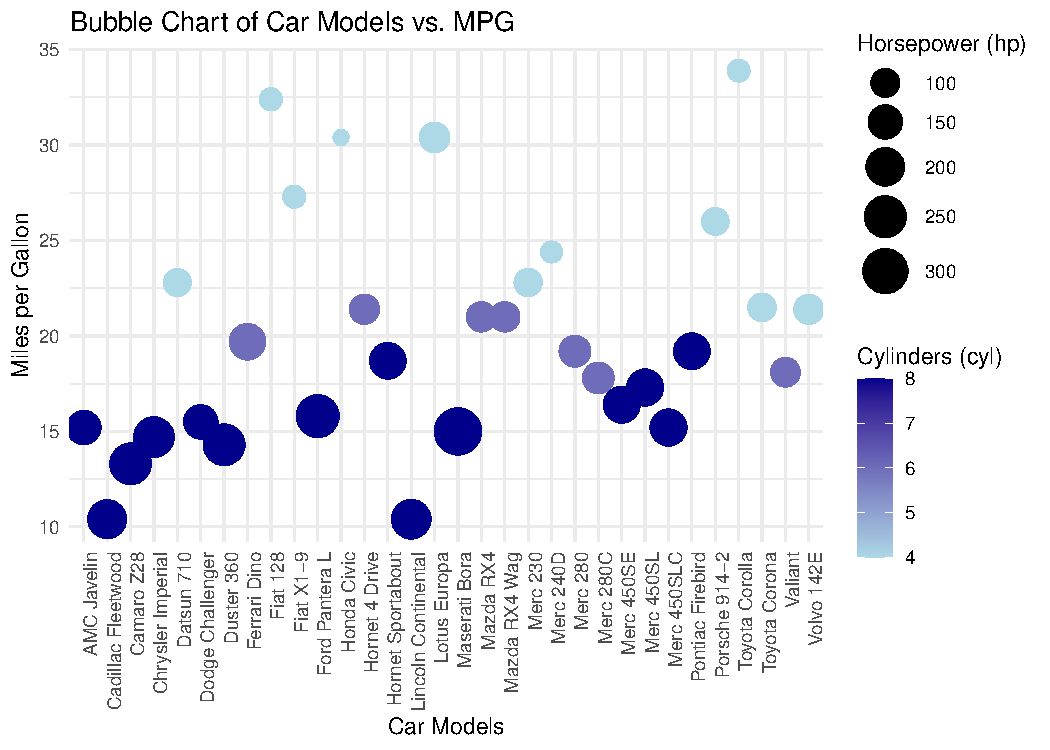
\includegraphics[width=\maxwidth]{figure/buble-plot-chunk-1} 
\end{knitrout}

\subsection{Key Considerations for Scatter Plots and Bubble Charts}
    \begin{enumerate}
        \item \textbf{Scaling}: Consider the scaling of the axes and bubble sizes to prevent distortion of the data representation.
        \item \textbf{Labeling}: Use clear labels, titles, and colour coding to make the visualisation more interpretable and meaning by decreasing the cognitive load. 
        \item \textbf{Interactivity}: Implement interactive features, such as tooltips or zooming, to allow users to explore individual data points in detail.
    \end{enumerate}


\section*{Chapter 3.3 Bar Charts and Histograms}
\subsection*{Bar Charts}
A bar chart is a very important method to present data. It organizes information into vertical bars.  Bar charts have lots of advantages in data visualization. It can present data categories in a frequency distribution. A bar chart is best for comparing classified data. Especially when the values are close, because the human perception of height is better than other visual elements (such as area, angle, etc.), the use of a bar chart is more appropriate. These bars usually have different lengths, and every length is proportional to the size of the information they present.\\
R uses the function $barplot()$ to create bar charts. R can draw both vertical and Horizontal bars in the bar chart. In the bar chart, each of the bars can be given different colors.\\
R is a programming language for data analysis and statistical computing, and its advent has made data visualization more straightforward and accessible. Among the various tools available in R, ggplot2 stands out as one of the most renowned and powerful tools for creating data visualizations. It offers a wealth of data visualization capabilities and is celebrated for its versatility and aesthetic appeal. In this chapter, we will focus on how to use ggplot2 to create bar charts for data visualization.\\

\subsection*{3.3.1 Different Types of Bar Charts}
Here is an overview of the different types of bar charts. \\
\paragraph{Vertical Bar Chart}
This is the most common bar chart. We use different vertical columns to display and compare the values of different categories in the same dimension, where the X-axis represents the contrasting categories and the Y-axis represents the frequency or count of their categories.\\
\paragraph{Horizontal Bar Chart}
This is very similar to a vertical bar chart but rotated 90 degrees. Categories are shown on the y-axis and frequency or count are shown on the x-axis. Horizontal bar charts are especially useful when category names are long or when there are numerous categories.
\paragraph{Multi-set Bar Chart}
Also known as a grouped bar chart or clustered bar chart. A multi-set bar chart is used to represent and compare different sub-groups within individual categories. This type of chart is useful when you want to show and compare multiple sets of data side-by-side.
Multi-set Bar charts can be horizontal or vertical like the other normal bar charts, and the length of each bar represents the frequency or count of their categories.
\paragraph{Stacked bar chart}
Similar to bar charts, stacked bar charts are often used to compare different classes of values and, within each class of values, are divided into sub-classes, which are often referred to by different colors. Each segment's size is proportional to the frequency or count that it represents from the sub-category. The entire bar's length represents the cumulative total of all the sub-categories.
However, it is very easy to get confused when there are too many categories.

\subsection*{3.3.2 Advantages of Bar Charts}
\begin{enumerate}
\item \textbf{Clarity and Simplicity}: Bar charts are structurally simple, making them easy to read and understand, allowing audiences to quickly grasp key information.
    \item \textbf{Effective Comparison}: They provide a visual representation that makes comparing the size or value of different categories straightforward, especially when comparing a limited number of categorical data.
    \item \textbf{High Flexibility}: They can be used to represent any type of data, be it continuous or discrete.
    \item \textbf{Multilevel Representation}: Stacked or grouped bar charts can be used to represent multiple data series.
\end{enumerate}

\subsection*{3.3.3 Disadvantages of Bar Charts}
\begin{enumerate}
    \item \textbf{Limited Data Representation}: They might not be suitable for representing large datasets as things can get cluttered.
    \item \textbf{Potential Misinterpretation}: Without a zero baseline, bar charts can be misleading as they might exaggerate differences.
    \item \textbf{Overcomplexity with Many Categories}: If there are too many bars, it can be challenging to discern information effectively.
    \item \textbf{Requires Categorical Data}: Bar charts are not ideal for representing trends over continuous data, where line graphs might be more appropriate.
\end{enumerate}

In this section, I will analyze the air quality dataset provided by the United States Environmental Protection Agency. In our dataset, we have data from over 200 locations. The Air Quality Index (AQI) ranges from 0 to 500. A higher AQI indicates increased levels of air pollution, leading to heightened health concerns. This implies that as the AQI rises, there is a greater risk to public health.

\begin{knitrout}
\definecolor{shadecolor}{rgb}{0.969, 0.969, 0.969}\color{fgcolor}\begin{kframe}
\begin{alltt}
\hlstd{data} \hlkwb{<-} \hlkwd{read.csv}\hlstd{(}\hlstr{"c4_epa_air_quality.csv"}\hlstd{)}
\hlkwd{ggplot}\hlstd{(data,} \hlkwd{aes}\hlstd{(}\hlkwc{x} \hlstd{= aqi))} \hlopt{+}
  \hlkwd{geom_bar}\hlstd{()} \hlopt{+}
  \hlkwd{labs}\hlstd{(}\hlkwc{title} \hlstd{=} \hlstr{"Bar Chart Example 1"}\hlstd{,} \hlkwc{x} \hlstd{=}
         \hlstr{"Air Quality Index/units"}\hlstd{,} \hlkwc{y} \hlstd{=} \hlstr{"number/sites"}\hlstd{)} \hlopt{+}
  \hlkwd{theme_minimal}\hlstd{()}
\end{alltt}
\end{kframe}
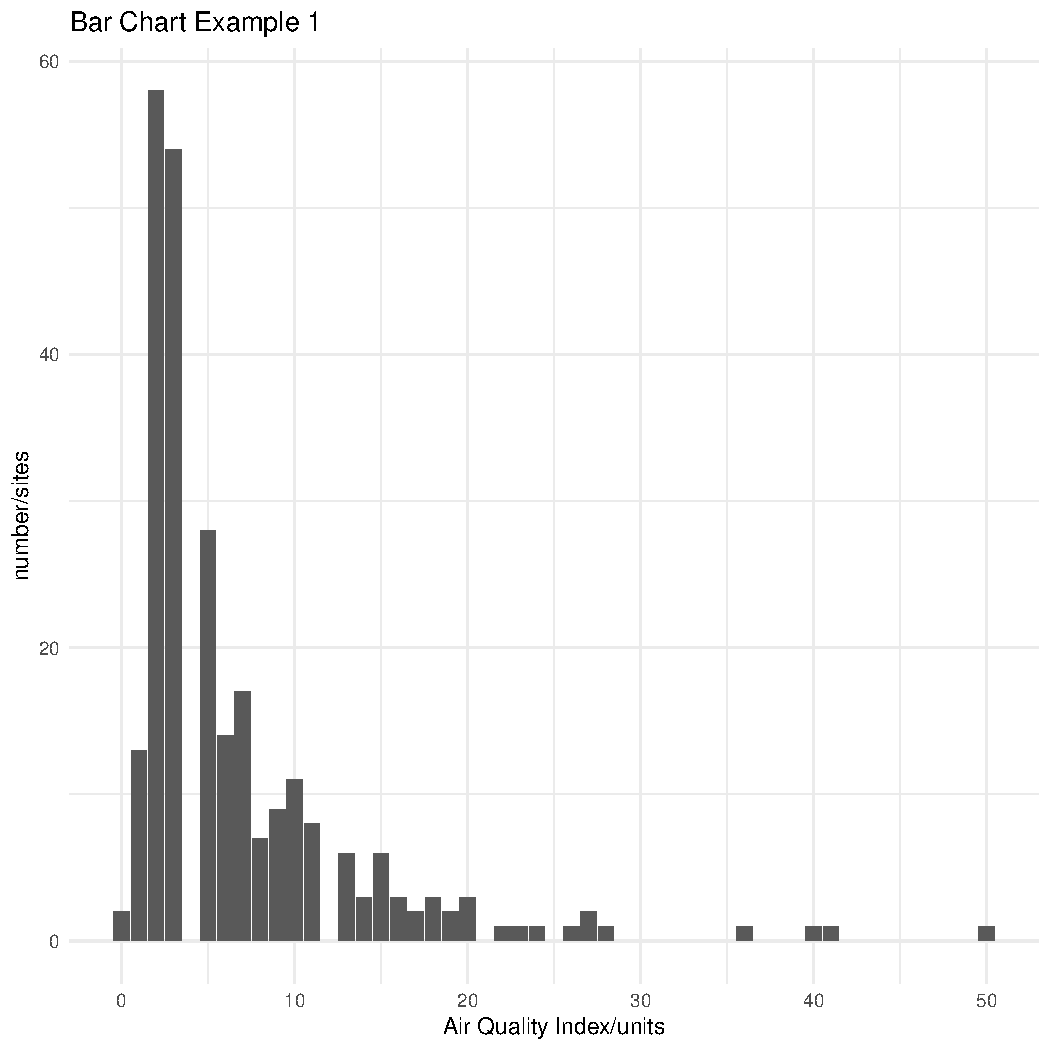
\includegraphics[width=\maxwidth]{figure/my_plot1-1} 
\end{knitrout}

The above code is not optimal. Upon examinationan, we can see that there is an excussive number of different categories on the x-axis. Consequently, the multitude of vertical bars in the graph can potentially overwhelm and confuse readers. 
In order to solve the problem, we can use the “cut” function to divide the data into intervals of five units each. For instance, values from 0-5 would constitute one group, 6-10 another, 11-15 would form the next group, and so forth.


\begin{knitrout}
\definecolor{shadecolor}{rgb}{0.969, 0.969, 0.969}\color{fgcolor}\begin{kframe}
\begin{alltt}
\hlstd{data} \hlkwb{<-} \hlkwd{read.csv}\hlstd{(}\hlstr{"c4_epa_air_quality.csv"}\hlstd{)} \hlcom{#}
\hlcom{# load ggplot2 package}
\hlkwd{library}\hlstd{(ggplot2)}

\hlcom{# Use the cut function to divide the data into groups of five intervals}
\hlstd{data}\hlopt{$}\hlstd{group} \hlkwb{<-} \hlkwd{cut}\hlstd{(data}\hlopt{$}\hlstd{aqi,} \hlkwc{breaks} \hlstd{=}
                    \hlkwd{seq}\hlstd{(}\hlnum{0}\hlstd{,} \hlkwd{max}\hlstd{(data}\hlopt{$}\hlstd{aqi)} \hlopt{+} \hlnum{5}\hlstd{,} \hlkwc{by} \hlstd{=} \hlnum{5}\hlstd{),}
                  \hlkwc{right} \hlstd{=} \hlnum{FALSE}\hlstd{,} \hlkwc{include.lowest} \hlstd{=} \hlnum{TRUE}\hlstd{)}
\hlstd{data}\hlopt{$}\hlstd{group} \hlkwb{<-} \hlkwd{as.numeric}\hlstd{(data}\hlopt{$}\hlstd{group)}

\hlcom{# Y-axis representing the number of occurrences of the X-axis label in the data}
\hlkwd{ggplot}\hlstd{(data,} \hlkwd{aes}\hlstd{(}\hlkwc{x} \hlstd{= group))} \hlopt{+}
  \hlkwd{geom_bar}\hlstd{()} \hlopt{+}
  \hlkwd{labs}\hlstd{(}\hlkwc{title} \hlstd{=} \hlstr{"Bar Chart Example 1"}\hlstd{,}
       \hlkwc{x} \hlstd{=} \hlstr{"Air Quality Index/units"}\hlstd{,} \hlkwc{y} \hlstd{=} \hlstr{"Number/sites"}\hlstd{)} \hlopt{+}
  \hlkwd{theme_minimal}\hlstd{()} \hlopt{+}
  \hlkwd{scale_x_discrete}\hlstd{(}\hlkwc{labels} \hlstd{= scales}\hlopt{::}\hlkwd{label_number}\hlstd{(}\hlkwc{accuracy} \hlstd{=} \hlnum{5}\hlstd{))}
\end{alltt}
\end{kframe}
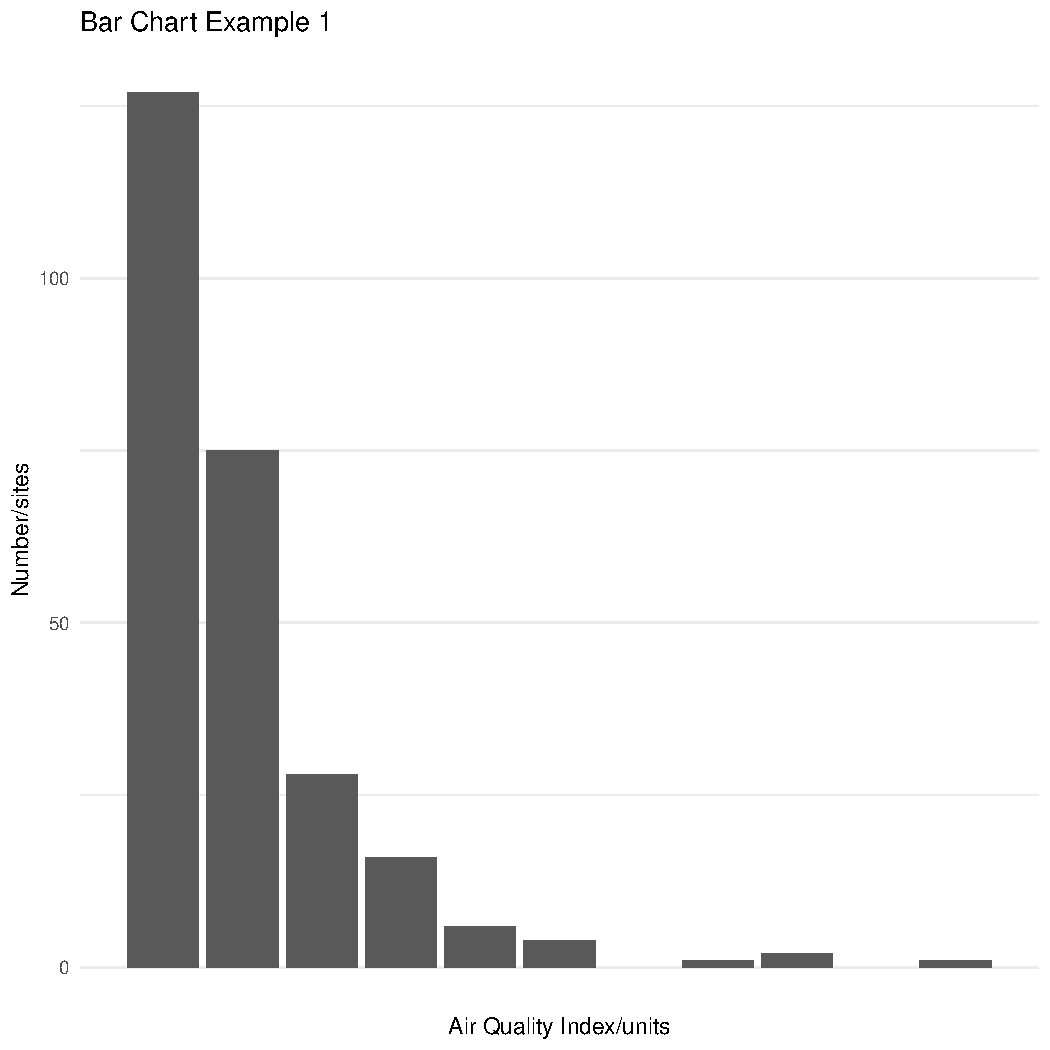
\includegraphics[width=\maxwidth]{figure/my_plot2-1} 
\end{knitrout}

We can also add some color to make our plot more attractive, here we can add sone color as well. In the code below, we set the color of the bar chart to blue while specifying the border color as black.

\begin{knitrout}
\definecolor{shadecolor}{rgb}{0.969, 0.969, 0.969}\color{fgcolor}\begin{kframe}
\begin{alltt}
\hlcom{# read CSV dater set}
\hlstd{data} \hlkwb{<-} \hlkwd{read.csv}\hlstd{(}\hlstr{"c4_epa_air_quality.csv"}\hlstd{)}

\hlcom{# load ggplot2 }
\hlkwd{library}\hlstd{(ggplot2)}

\hlcom{# Use the cut function to divide the data into groups of five intervals}
\hlstd{data}\hlopt{$}\hlstd{group} \hlkwb{<-} \hlkwd{cut}\hlstd{(data}\hlopt{$}\hlstd{aqi,} \hlkwc{breaks} \hlstd{=} \hlkwd{seq}\hlstd{(}\hlnum{0}\hlstd{,} \hlkwd{max}\hlstd{(data}\hlopt{$}\hlstd{aqi)} \hlopt{+} \hlnum{5}\hlstd{,} \hlkwc{by} \hlstd{=} \hlnum{5}\hlstd{),}
                  \hlkwc{right} \hlstd{=} \hlnum{FALSE}\hlstd{,} \hlkwc{include.lowest} \hlstd{=} \hlnum{TRUE}\hlstd{)}
\hlstd{data}\hlopt{$}\hlstd{group} \hlkwb{<-} \hlkwd{as.numeric}\hlstd{(data}\hlopt{$}\hlstd{group)}
\hlcom{# Converts the group column to numeric type}

\hlkwd{ggplot}\hlstd{(data,} \hlkwd{aes}\hlstd{(}\hlkwc{x} \hlstd{= group))} \hlopt{+}
  \hlkwd{geom_bar}\hlstd{(}\hlkwc{color}\hlstd{=}\hlstr{"black"}\hlstd{,}\hlkwc{fill}\hlstd{=}\hlstr{"blue"}\hlstd{)} \hlopt{+}
  \hlkwd{labs}\hlstd{(}\hlkwc{title} \hlstd{=} \hlstr{"Bar Chart Example 1"}\hlstd{,} \hlkwc{x} \hlstd{=} \hlstr{"Air Quality Index/units"}\hlstd{,}
       \hlkwc{y} \hlstd{=} \hlstr{"Number/sites"}\hlstd{)} \hlopt{+}
  \hlkwd{theme_minimal}\hlstd{()} \hlopt{+}
  \hlkwd{scale_x_discrete}\hlstd{(}\hlkwc{labels} \hlstd{= scales}\hlopt{::}\hlkwd{label_number}\hlstd{(}\hlkwc{accuracy} \hlstd{=} \hlnum{5}\hlstd{))}
\end{alltt}
\end{kframe}
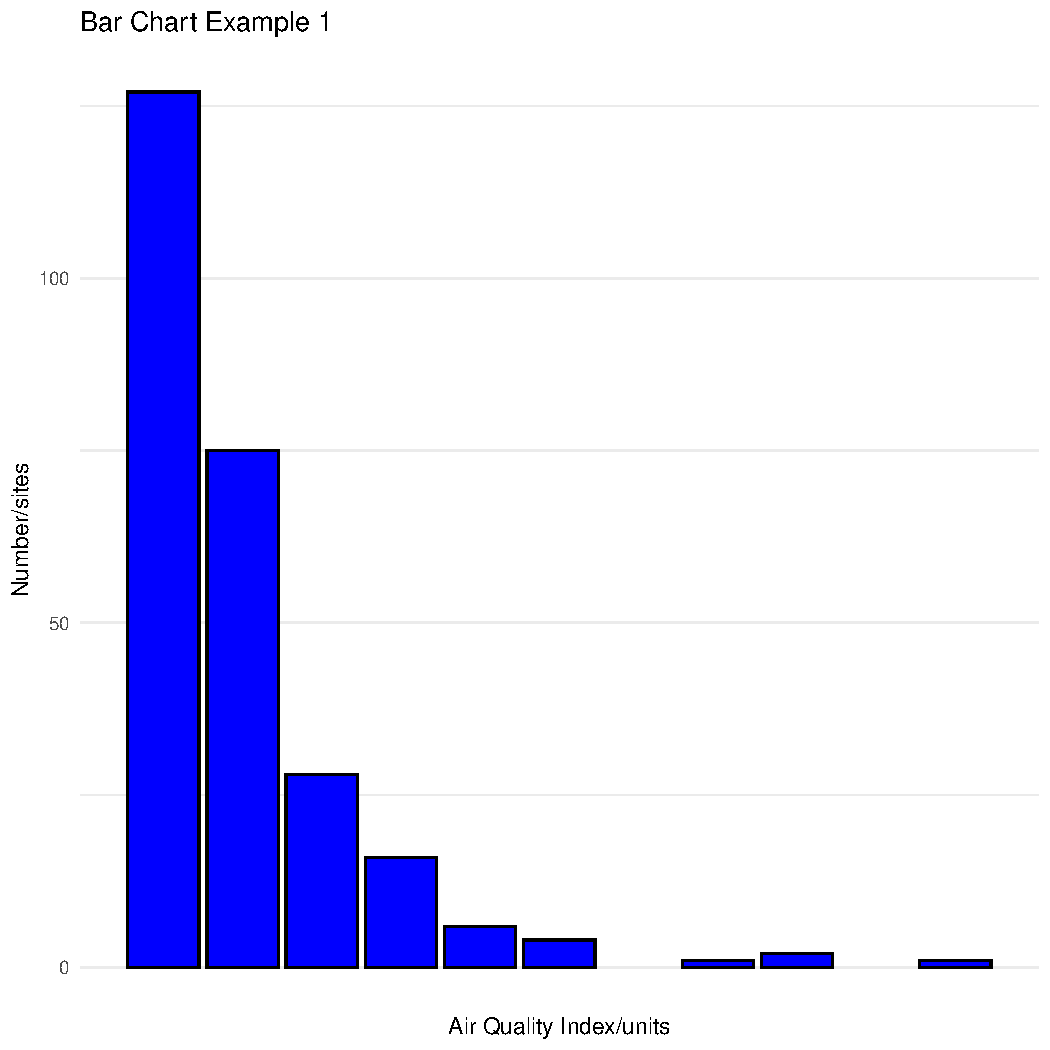
\includegraphics[width=\maxwidth]{figure/my_plot3-1} 
\end{knitrout}

Finally, we add lables to the X-axis to define the range of each categories.
\begin{knitrout}
\definecolor{shadecolor}{rgb}{0.969, 0.969, 0.969}\color{fgcolor}\begin{kframe}
\begin{alltt}
\hlcom{# read csv}
\hlstd{data} \hlkwb{<-} \hlkwd{read.csv}\hlstd{(}\hlstr{"c4_epa_air_quality.csv"}\hlstd{)}

\hlcom{# load ggplot2}
\hlkwd{library}\hlstd{(ggplot2)}

\hlcom{# Use the cut function to divide the data into groups of five intervals}
\hlstd{breaks_list} \hlkwb{<-} \hlkwd{seq}\hlstd{(}\hlnum{0}\hlstd{,} \hlkwd{max}\hlstd{(data}\hlopt{$}\hlstd{aqi)} \hlopt{+} \hlnum{5}\hlstd{,} \hlkwc{by} \hlstd{=} \hlnum{5}\hlstd{)}
\hlstd{data}\hlopt{$}\hlstd{group} \hlkwb{<-} \hlkwd{cut}\hlstd{(data}\hlopt{$}\hlstd{aqi,} \hlkwc{breaks} \hlstd{= breaks_list,}
                  \hlkwc{right} \hlstd{=} \hlnum{FALSE}\hlstd{,} \hlkwc{include.lowest} \hlstd{=} \hlnum{TRUE}\hlstd{)}


\hlkwd{ggplot}\hlstd{(data,} \hlkwd{aes}\hlstd{(}\hlkwc{x} \hlstd{= group))} \hlopt{+}
  \hlkwd{geom_bar}\hlstd{(}\hlkwc{color}\hlstd{=}\hlstr{"black"}\hlstd{,} \hlkwc{fill}\hlstd{=}\hlstr{"blue"}\hlstd{)} \hlopt{+}
  \hlkwd{labs}\hlstd{(}\hlkwc{title} \hlstd{=} \hlstr{"Bar Chart Example 2"}\hlstd{,} \hlkwc{x} \hlstd{=} \hlstr{"Air Quality Index/units"}\hlstd{,}
       \hlkwc{y} \hlstd{=} \hlstr{"Number/sites"}\hlstd{)} \hlopt{+}
  \hlkwd{theme_minimal}\hlstd{()} \hlopt{+}
  \hlkwd{scale_x_discrete}\hlstd{(}\hlkwc{labels} \hlstd{=} \hlkwd{paste0}
                   \hlstd{(breaks_list[}\hlopt{-}\hlkwd{length}\hlstd{(breaks_list)],} \hlstr{"-"}\hlstd{, breaks_list[}\hlopt{-}\hlnum{1}\hlstd{]))}
\end{alltt}
\end{kframe}
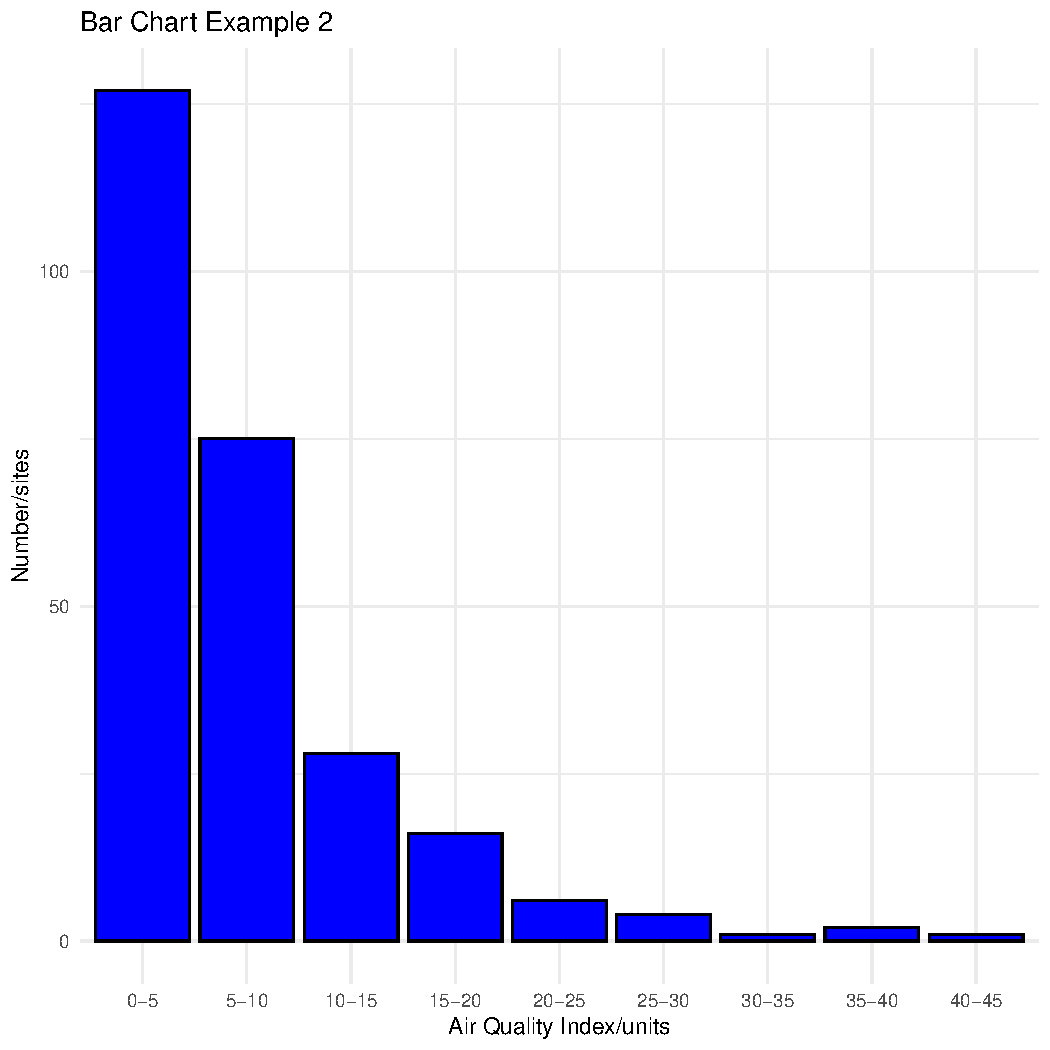
\includegraphics[width=\maxwidth]{figure/my_plot4-1} 
\end{knitrout}

\section{Chapter 3.4 Heatmaps and Tree Maps}





\begin{knitrout}
\definecolor{shadecolor}{rgb}{0.969, 0.969, 0.969}\color{fgcolor}\begin{kframe}
\begin{alltt}
\hlcom{# Obtain the Brazil map data}
\hlstd{brazil_map} \hlkwb{<-} \hlkwd{map_data}\hlstd{(}\hlstr{"world"}\hlstd{,} \hlkwc{region} \hlstd{=} \hlstr{"Brazil"}\hlstd{)}

\hlcom{# Create the heatmap of fire occurrences}
\hlstd{fire_heatmap} \hlkwb{<-} \hlkwd{ggplot}\hlstd{(confident_fire_fy22,} \hlkwd{aes}\hlstd{(}\hlkwc{x} \hlstd{= longitude,} \hlkwc{y} \hlstd{= latitude))} \hlopt{+}
  \hlkwd{geom_polygon}\hlstd{(}\hlkwc{data} \hlstd{= brazil_map,} \hlkwd{aes}\hlstd{(}\hlkwc{x} \hlstd{= long,} \hlkwc{y} \hlstd{= lat,} \hlkwc{group} \hlstd{= group),}
               \hlkwc{fill} \hlstd{=} \hlstr{"#bdbdbd"}\hlstd{)} \hlopt{+}
  \hlkwd{geom_bin2d}\hlstd{(}\hlkwc{bins} \hlstd{=} \hlnum{300}\hlstd{)} \hlopt{+}
  \hlkwd{scale_fill_gradient}\hlstd{(}\hlkwc{low} \hlstd{=} \hlstr{"#fee6ce"}\hlstd{,} \hlkwc{high} \hlstd{=} \hlstr{"#d94801"}\hlstd{)} \hlopt{+}
  \hlkwd{coord_fixed}\hlstd{(}\hlkwc{ratio} \hlstd{=} \hlnum{1}\hlstd{)} \hlopt{+}
  \hlkwd{labs}\hlstd{(}\hlkwc{title} \hlstd{=} \hlstr{"Frequency of Fire Occurrences by location in FY22"}\hlstd{)}

\hlkwd{print}\hlstd{(fire_heatmap)}
\end{alltt}
\end{kframe}
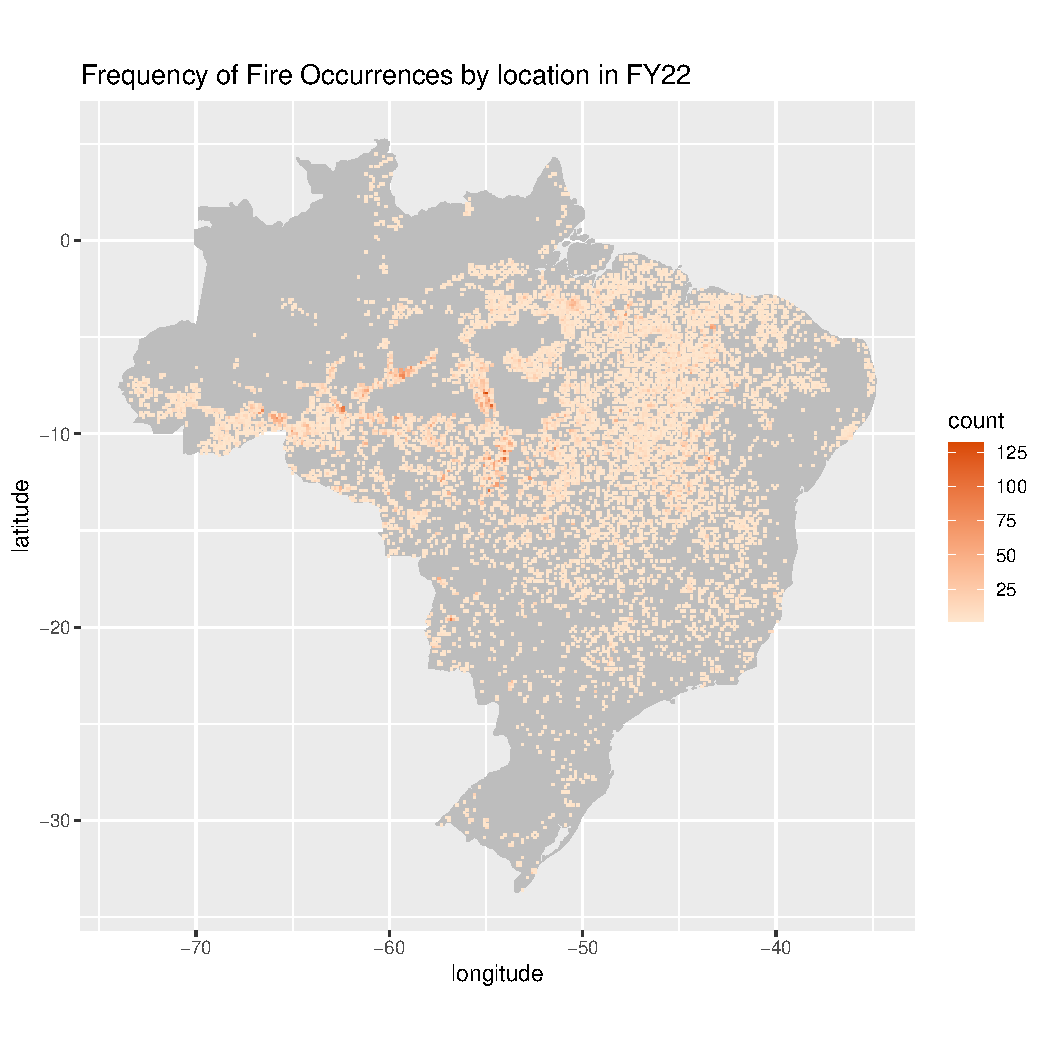
\includegraphics[width=\maxwidth]{figure/fire-by-location-fy22-1} 
\begin{kframe}\begin{alltt}
\hlcom{# Colour selection from: https://colorbrewer2.org/#type=sequential&scheme=Oranges&n=9}
\end{alltt}
\end{kframe}
\end{knitrout}



\begin{knitrout}
\definecolor{shadecolor}{rgb}{0.969, 0.969, 0.969}\color{fgcolor}\begin{kframe}
\begin{alltt}
\hlstd{heatmap_plot} \hlkwb{<-} \hlkwd{ggplot}\hlstd{(confident_fire_months_fy22,}
                       \hlkwd{aes}\hlstd{(}\hlkwc{x} \hlstd{= abb_month,} \hlkwc{y} \hlstd{=} \hlnum{2022}\hlstd{,} \hlkwc{fill} \hlstd{= count))} \hlopt{+}
  \hlkwd{geom_tile}\hlstd{(}\hlkwc{width} \hlstd{=} \hlnum{0.9}\hlstd{,} \hlkwc{height} \hlstd{=} \hlnum{1}\hlstd{)} \hlopt{+}  \hlcom{# Create the heatmap tiles}
  \hlkwd{scale_fill_gradient}\hlstd{(}\hlkwc{low} \hlstd{=} \hlstr{"white"}\hlstd{,} \hlkwc{high} \hlstd{=} \hlstr{"#d94801"}\hlstd{)} \hlopt{+}  \hlcom{# Customize the color scale}
  \hlkwd{labs}\hlstd{(}\hlkwc{title} \hlstd{=} \hlstr{"Frequency of Fire Occurrences by months in FY22"}\hlstd{,} \hlkwc{x} \hlstd{=} \hlstr{"Month"}\hlstd{,} \hlkwc{y} \hlstd{=} \hlstr{"FY22"}\hlstd{)} \hlopt{+}
  \hlkwd{theme}\hlstd{(}\hlkwc{panel.grid} \hlstd{=} \hlkwd{element_blank}\hlstd{() )}

\hlcom{# Display the heatmap}
\hlkwd{print}\hlstd{(heatmap_plot)}
\end{alltt}
\end{kframe}
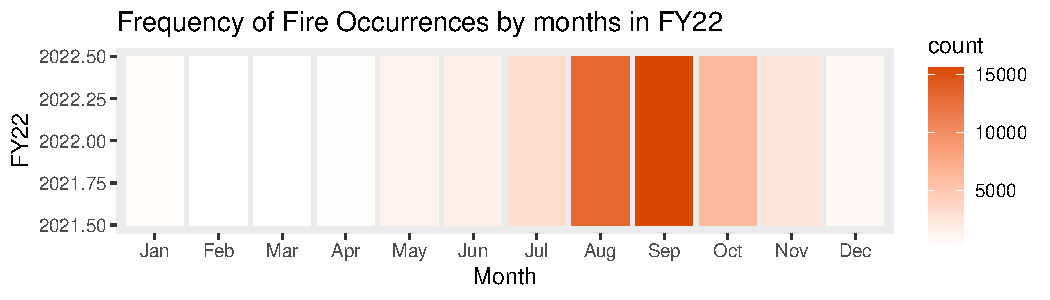
\includegraphics[width=\maxwidth]{figure/fire-by-months_fy22-1} 
\end{knitrout}
From the table, we can clearly see that August and September are the riskiest months in terms of fire hazard, whereas November to July hardly pose any risk at all. It's natural to ask the follow-up question: How does FY22 compare to previous years? Is it valid to claim that August and September are the fire hazard season?


\section*{Chapter 3.5 Line Charts and Time Series Visualization}

A \textbf{Line chart}, often referred to as a line graph or line plot, is a statistical chart composed of a Cartesian coordinate system, some points, and lines. It is commonly used to represent changes in numerical values over continuous time intervals or ordered categories. In a line graph, the x-axis is typically used for continuous time intervals or ordered categories (such as Stage 1, Stage 2, Stage 3). The y-axis is used for quantified data, and if it is negative, it is plotted below the y-axis. Lines are used to connect adjacent data points.

Line graphs are used to analyze trends in things that change over time or ordered categories. If there are multiple sets of data, they are used to analyze the interaction and impact of these data sets over time or ordered categories. The direction of the line represents positive/negative changes, and the slope of the line indicates the degree of change.

In terms of data, a line graph requires a continuous time field or a categorical field and at least one continuous data field.


\subsection{Basic Components}
\begin{itemize}
  \item \textbf{X-Axis (Horizontal Axis):} Typically represents the independent variable, such as time or date.
  \item \textbf{Y-Axis (Vertical Axis):} Typically represents the dependent variable, like sales numbers, stock prices, or temperatures.
  \item \textbf{Line:} Connects the individual data points. In some line charts, multiple lines can represent different categories or sets of data.
\end{itemize}


\subsection{Suitability for Displaying Trends Over Time:}
\begin{itemize}
    \item \textbf{Visual Clarity:} Line charts provide a clear and concise way to view changes over time. When data points are plotted over regular intervals (e.g., days, months, years), it becomes easy to see upward or downward trends.
    \item \textbf{Comparisons:} When you have multiple lines on a single chart, you can easily compare different sets of data. For instance, comparing sales data of two different products over time.
    \item \textbf{Identification of Patterns:} Line charts help in identifying patterns and anomalies. Seasonal patterns, cyclical events, and unexpected spikes or dips become evident.
    \item \textbf{Forecasting:} By viewing historical data trends on a line chart, analysts can make predictions or forecasts for future data points.
    \item \textbf{Simplicity:} They are easy to understand and interpret. Even if someone isn't data-savvy, they can grasp the general trend and major fluctuations from a line chart.
    \item \textbf{Flexibility:} They can be used for both short-term and long-term data. Whether you're looking at stock prices minute-by-minute over a single day or global temperature averages over a century, line charts can effectively represent the data.
\end{itemize}


\subsection{Limitations:}
While line charts are excellent for displaying trends over time, they have limitations. They may not be suitable for showing individual data distributions or for data where there's no logical order. eg. too many points, too many lines, too many zeros.\\


\subsection*{Discuss the importance of time series visualisation in data analysis.}

Time series visualization refers to the graphical representation of time-ordered data points. In the world of data analysis, this form of visualization is invaluable for examining patterns, anomalies, and trends in datasets that evolve over time.\\
\textbf{Uncovering Trends:}\\
One of the primary advantages of time series visualization is the ease with which it allows analysts to identify long-term upward or downward trends in data. Recognizing these trends can help organizations make informed decisions about future strategies or interventions.\\
\textbf{Detection of Seasonality:}\\
Many datasets exhibit patterns that repeat over specific intervals, such as days, months, or years. Time series visualization makes it straightforward to spot such cyclical behaviors, which can be vital for businesses in sectors like retail or agriculture.\\
\textbf{Identifying Anomalies:}\\
Graphical representations can quickly highlight data points or periods that deviate significantly from the norm. These anomalies can indicate errors in data collection, or they may reveal significant events that need to be further investigated.\\
\textbf{Forecasting and Predictions:}\\
After identifying patterns in historical data, time series visualizations can aid in modeling future data points. Predictive modeling, underpinned by clear visualizations, allows businesses to make proactive decisions.\\
\textbf{Facilitating Comparative Analysis:}\\
Time series charts often allow for overlaying multiple data series on a single graph. This capability is useful for comparing different datasets or the same dataset under different conditions, leading to more comprehensive insights.\\
\textbf{Conclusion:}\\
Time series visualization is an indispensable tool in the arsenal of data analysts. It condenses large volumes of chronological data into easily interpretable graphics, enabling quick insights, better decision-making, and a deeper understanding of temporal dynamics in datasets. By providing a clear view of data trends, seasonality, and anomalies, time series visualization facilitates more informed and strategic actions in various domains.



\section*{Provide best practices for creating clear and informative line charts.}

\begin{itemize}
  \item Title and Labels: Every chart should have a descriptive title and axis labels to clearly convey the purpose of the visualization and the data being shown.
  \item Use of Colors: Colors should be chosen to clearly differentiate between different lines or data points but also be consistent with the overall theme or style.
  \item Gridlines and Background: Soft gridlines can help the viewer estimate values. A clean background aids in clarity.
  \item Line Types and Point Shapes: When multiple lines are on the same chart, use different line types and point shapes to differentiate between them.
  \item Consistent Scaling: The scale on the y-axis should be consistent so that the viewer isn't misled.
  \item Annotations: Important points or changes can be annotated directly on the graph.
  \item Legends: If there are multiple lines or data points with different colors/shapes, a legend should be provided.
\end{itemize}

Let's apply these practices:


First, we generate 2 series of random data.

\begin{knitrout}
\definecolor{shadecolor}{rgb}{0.969, 0.969, 0.969}\color{fgcolor}\begin{kframe}
\begin{alltt}
\hlstd{x} \hlkwb{<-} \hlkwd{seq}\hlstd{(}\hlnum{1}\hlstd{,} \hlnum{20}\hlstd{)}
\hlstd{y} \hlkwb{<-} \hlkwd{runif}\hlstd{(}\hlnum{20}\hlstd{)}
\hlstd{data} \hlkwb{<-} \hlkwd{data.frame}\hlstd{(}\hlkwc{x} \hlstd{= x,} \hlkwc{y} \hlstd{= y)}
\end{alltt}
\end{kframe}
\end{knitrout}

Below is a line chart of the random sample:

\begin{knitrout}
\definecolor{shadecolor}{rgb}{0.969, 0.969, 0.969}\color{fgcolor}
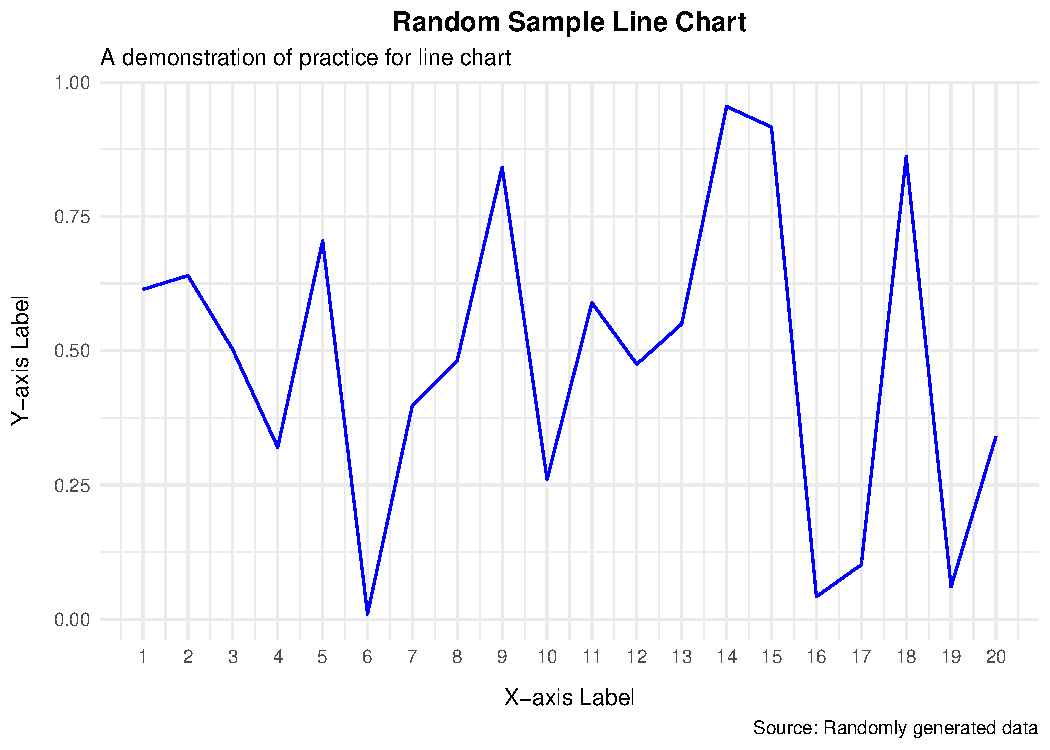
\includegraphics[width=\maxwidth]{figure/plot-chunk-1} 
\end{knitrout}


\section*{Showcase real-world examples of time series visualisations.}

Time series of the daily CNY, CAN, EUR, HKD, USD versus GBP exchange reference rate data
published by the European Central Bank over the time period from 01 Jan 2013 to 12 Oct 2023 (without weekends). The exchange rate tells you how many pounds you need to buy/sell 1 CNY, CAN, EUR, HKD, USD.

\subsection{The data set has the format as below:}

\begin{table}[h]
\centering
\begin{tabular}{|c|c|c|c|c|c|}
\hline
\textbf{Date} & \textbf{CNYtoGBP} & \textbf{CANtoGBP} & \textbf{EURtoGBP} & \textbf{HKDtoGBP} & \textbf{USDtoGBP} \\
\hline
\%d-\%m-\%y & Value & Value & Value & Value & Value \\
\hline
& & & & & \\
\hline
\end{tabular}
\caption{Field Information: CNY, CAN, EUR, HKD, USD to GBP}
\end{table}


\subsection{Multiple time series in one plot:}

\begin{knitrout}
\definecolor{shadecolor}{rgb}{0.969, 0.969, 0.969}\color{fgcolor}
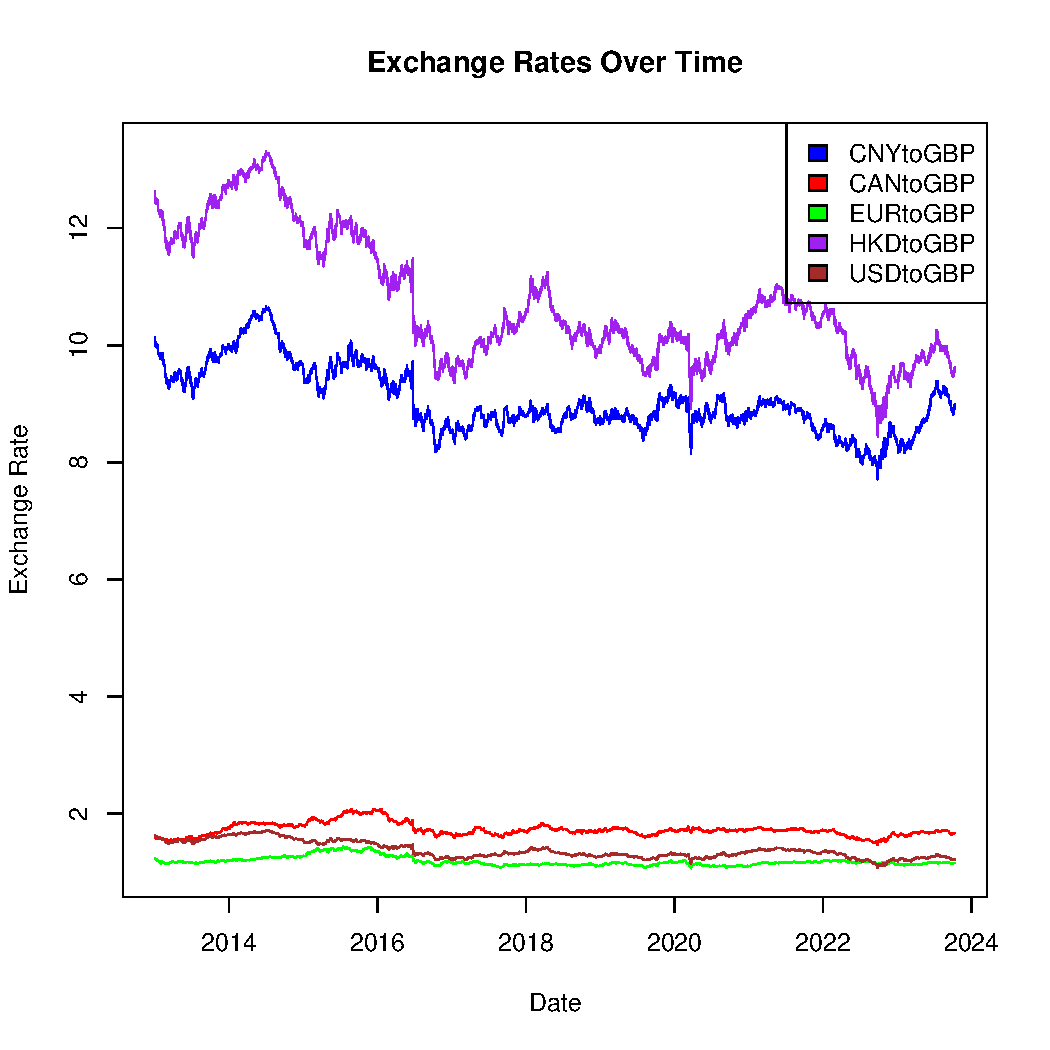
\includegraphics[width=\maxwidth]{figure/unnamed-chunk-1-1} 
\end{knitrout}

\subsection{Decomposition of one time series into trend, seasonal, and random.}


One of the primary advantages of time series visualization is the ease with which it allows analysts to identify long-term upward or downward trends in data and patterns that repeat over specific intervals. By decomposing the time series, it would be easy to see those features.

\begin{knitrout}
\definecolor{shadecolor}{rgb}{0.969, 0.969, 0.969}\color{fgcolor}
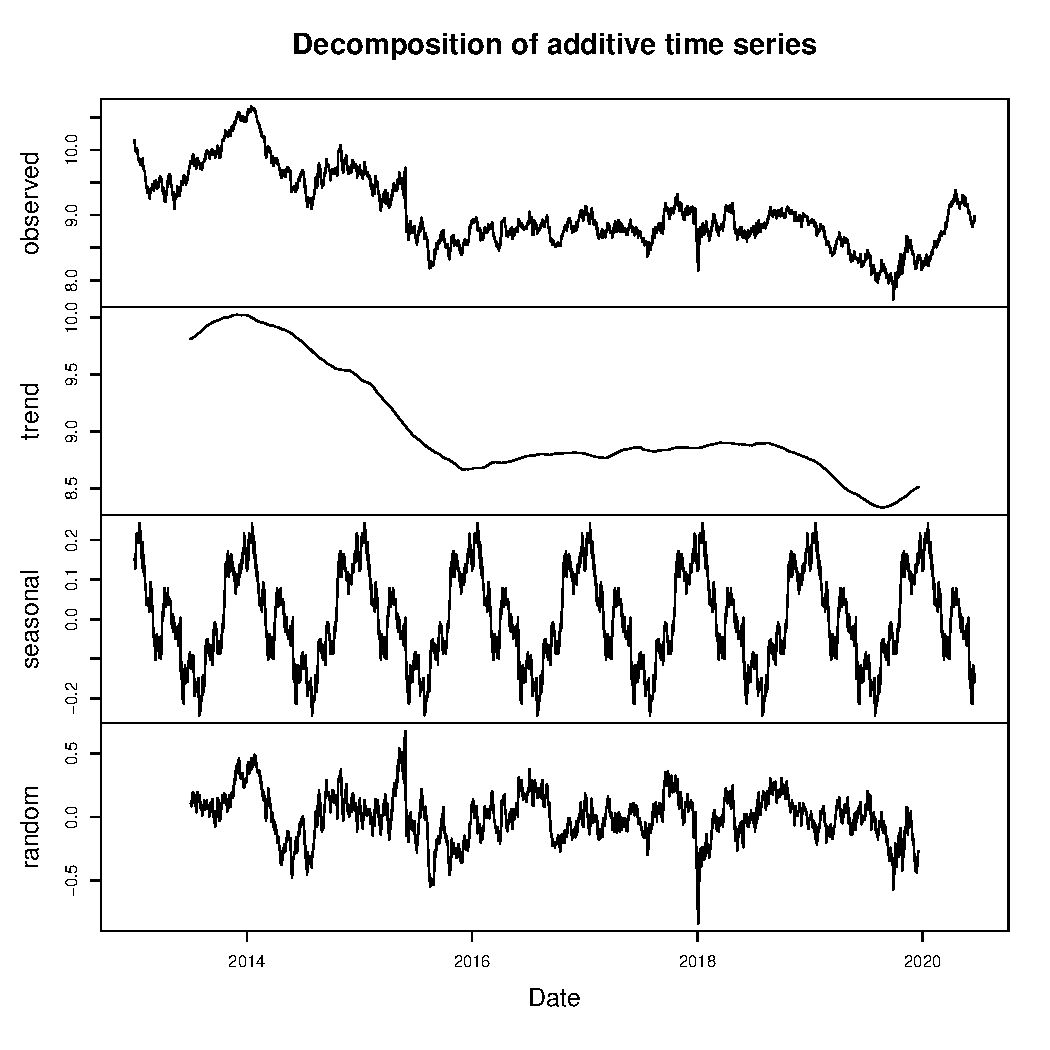
\includegraphics[width=\maxwidth]{figure/unnamed-chunk-2-1} 
\end{knitrout}


\subsection{Double y-axis time series plot.}

If we want to display two different time series that measure two different quantities at the same time points, we can draw the second series again on the second Y-axis on the right side.

\begin{knitrout}
\definecolor{shadecolor}{rgb}{0.969, 0.969, 0.969}\color{fgcolor}
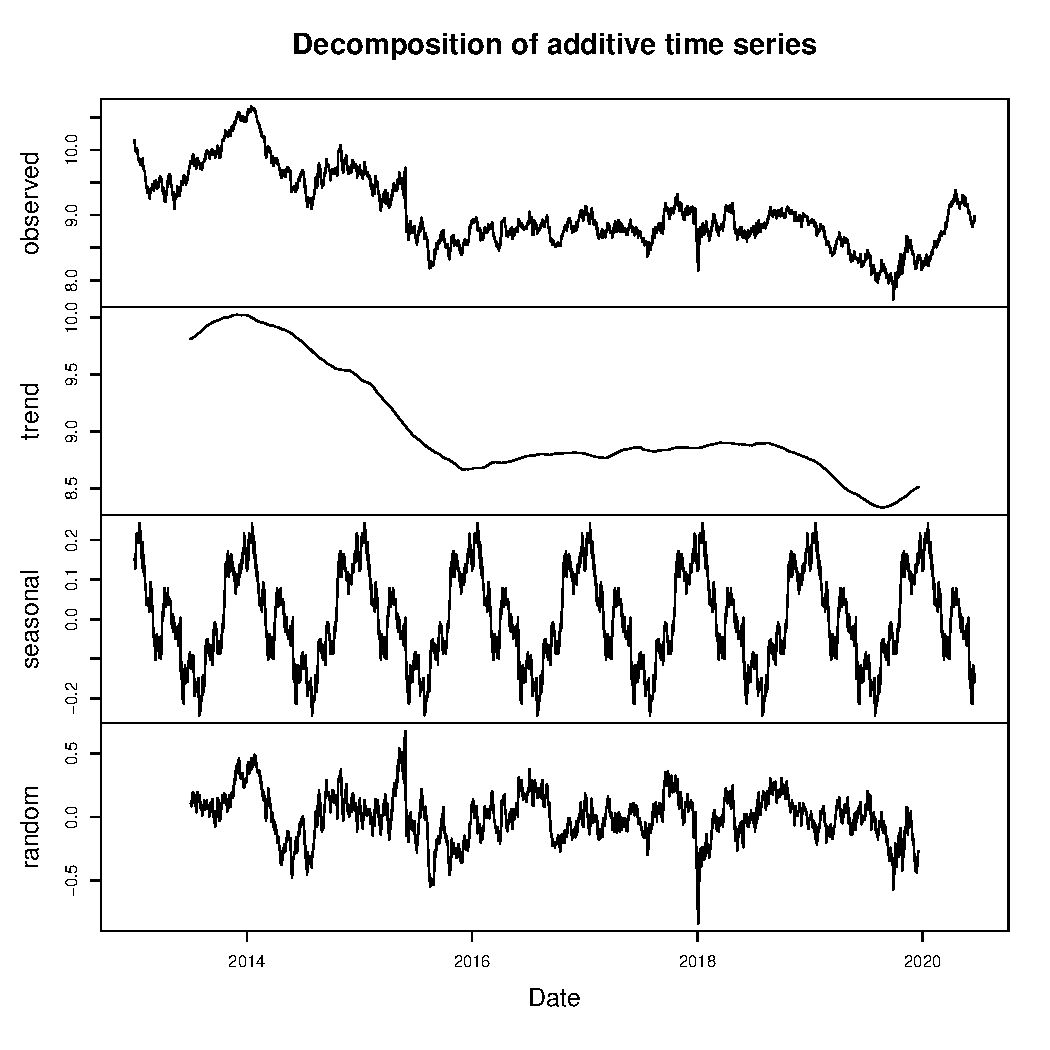
\includegraphics[width=\maxwidth]{figure/unnamed-chunk-3-1} 
\end{knitrout}


\section{Chapter 3.5 Network Graphs and Sankey Diagrams}
xxx

\section{Chapter 3.6 Geographic Maps and Spatial Data Visualisation}
xxx

\section{Chapter 3.7 3D and Interactive Visualisations}
xxx

\section{Chapter 3.8 Advanced Visualisation Techniques}
xxx


\end{document}
